\begin{Large}
    \textsf{\textbf{Program 2 - Pi Estimation by Acceptance Rejection Method}}
\end{Large}

\vspace{2em}

\header{Aim:} To estimate the value of $\pi$ to within a given precision using the acceptance-rejection method along with ensemble-averaging\\

In this method, a variation of which was proposed by Laplace in 1812, we actually estimate the volume of a circle $\mathcal{C}$ inscribed within the square region $\mathcal{S} = [-1,+1]\times[-1,+1] \subset \mathbb{R}^2 $

We sample two uniformly distributed numbers $x_i$, $y_i$, with the distribution scaled such that $x_i,y_i \in [-1,+1]\subset \mathbb{R}$. As the two samples are independent, we may regard a series of $N$ such pairs $(x_i,y_i)$ as uniformly distributed points in $\mathcal{S}$

Given that the distribution of points is uniform, we have for a given sampled point $p$:

\begin{align*}
    \textbf{Prob}(p\in \mathcal{C}) &= \frac{\textbf{Area}(\mathcal{C})}{\textbf{Area}(\mathcal{S})} \\
     &= \frac{\pi}{4}
\end{align*}

The probability in the above expression is estimated by the fraction of points out of $N$ that lie inside the circle. Thus we have

$$ \pi = 4\times\frac{\text{no. of points inside \mathcal{C}}}{N}$$

\begin{figure}[!htb]
    \centering
    

\tikzset{every picture/.style={line width=0.75pt}} %set default line width to 0.75pt        

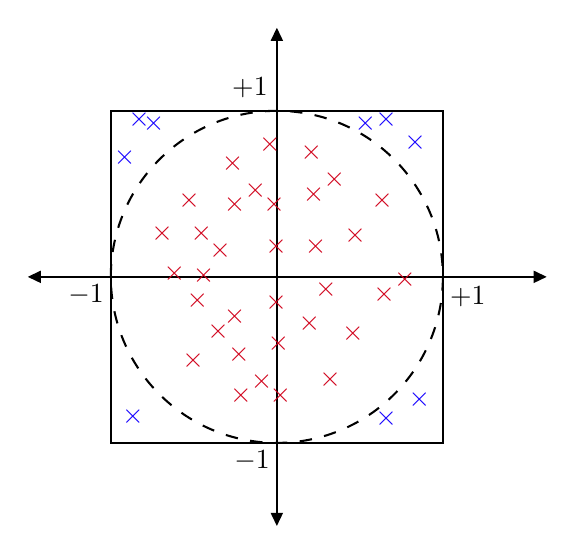
\begin{tikzpicture}[x=0.75pt,y=0.75pt,yscale=-1,xscale=1]
%uncomment if require: \path (0,311); %set diagram left start at 0, and has height of 311

%Shape: Rectangle [id:dp4502989580556914] 
\draw   (200,70) -- (360,70) -- (360,230) -- (200,230) -- cycle ;
%Straight Lines [id:da3211723360292128] 
\draw    (280,33) -- (280,101) -- (280,267) ;
\draw [shift={(280,270)}, rotate = 270] [fill={rgb, 255:red, 0; green, 0; blue, 0 }  ][line width=0.08]  [draw opacity=0] (6.25,-3) -- (0,0) -- (6.25,3) -- cycle    ;
\draw [shift={(280,30)}, rotate = 90] [fill={rgb, 255:red, 0; green, 0; blue, 0 }  ][line width=0.08]  [draw opacity=0] (6.25,-3) -- (0,0) -- (6.25,3) -- cycle    ;
%Straight Lines [id:da9614344093722763] 
\draw    (407,150) -- (163,150) ;
\draw [shift={(160,150)}, rotate = 360] [fill={rgb, 255:red, 0; green, 0; blue, 0 }  ][line width=0.08]  [draw opacity=0] (6.25,-3) -- (0,0) -- (6.25,3) -- cycle    ;
\draw [shift={(410,150)}, rotate = 180] [fill={rgb, 255:red, 0; green, 0; blue, 0 }  ][line width=0.08]  [draw opacity=0] (6.25,-3) -- (0,0) -- (6.25,3) -- cycle    ;
%Shape: Circle [id:dp6587946017419893] 
\draw  [dash pattern={on 4.5pt off 4.5pt}] (200,150) .. controls (200,105.82) and (235.82,70) .. (280,70) .. controls (324.18,70) and (360,105.82) .. (360,150) .. controls (360,194.18) and (324.18,230) .. (280,230) .. controls (235.82,230) and (200,194.18) .. (200,150) -- cycle ;

% Text Node
\draw (178,152.4) node [anchor=north west][inner sep=0.75pt]    {$-1$};
% Text Node
\draw (257,52.4) node [anchor=north west][inner sep=0.75pt]    {$+1$};
% Text Node
\draw (258,232.4) node [anchor=north west][inner sep=0.75pt]    {$-1$};
% Text Node
\draw (362,153.4) node [anchor=north west][inner sep=0.75pt]    {$+1$};
% Text Node
\draw (214,70.4) node [anchor=north west][inner sep=0.75pt]  [color={rgb, 255:red, 20; green, 0; blue, 255 }  ,opacity=1 ]  {$\times $};
% Text Node
\draw (200,86.4) node [anchor=north west][inner sep=0.75pt]  [color={rgb, 255:red, 20; green, 0; blue, 255 }  ,opacity=1 ]  {$\times $};
% Text Node
\draw (207,68.4) node [anchor=north west][inner sep=0.75pt]  [color={rgb, 255:red, 20; green, 0; blue, 255 }  ,opacity=1 ]  {$\times $};
% Text Node
\draw (342,203.4) node [anchor=north west][inner sep=0.75pt]  [color={rgb, 255:red, 20; green, 0; blue, 255 }  ,opacity=1 ]  {$\times $};
% Text Node
\draw (326,212.4) node [anchor=north west][inner sep=0.75pt]  [color={rgb, 255:red, 20; green, 0; blue, 255 }  ,opacity=1 ]  {$\times $};
% Text Node
\draw (204,211.4) node [anchor=north west][inner sep=0.75pt]  [color={rgb, 255:red, 20; green, 0; blue, 255 }  ,opacity=1 ]  {$\times $};
% Text Node
\draw (326,68.4) node [anchor=north west][inner sep=0.75pt]  [color={rgb, 255:red, 20; green, 0; blue, 255 }  ,opacity=1 ]  {$\times $};
% Text Node
\draw (340,79.4) node [anchor=north west][inner sep=0.75pt]  [color={rgb, 255:red, 20; green, 0; blue, 255 }  ,opacity=1 ]  {$\times $};
% Text Node
\draw (316,70.4) node [anchor=north west][inner sep=0.75pt]  [color={rgb, 255:red, 20; green, 0; blue, 255 }  ,opacity=1 ]  {$\times $};
% Text Node
\draw (290,84.4) node [anchor=north west][inner sep=0.75pt]  [color={rgb, 255:red, 208; green, 2; blue, 27 }  ,opacity=1 ]  {$\times $};
% Text Node
\draw (324,107.4) node [anchor=north west][inner sep=0.75pt]  [color={rgb, 255:red, 208; green, 2; blue, 27 }  ,opacity=1 ]  {$\times $};
% Text Node
\draw (291,104.4) node [anchor=north west][inner sep=0.75pt]  [color={rgb, 255:red, 208; green, 2; blue, 27 }  ,opacity=1 ]  {$\times $};
% Text Node
\draw (301,97.4) node [anchor=north west][inner sep=0.75pt]  [color={rgb, 255:red, 208; green, 2; blue, 27 }  ,opacity=1 ]  {$\times $};
% Text Node
\draw (311,124.4) node [anchor=north west][inner sep=0.75pt]  [color={rgb, 255:red, 208; green, 2; blue, 27 }  ,opacity=1 ]  {$\times $};
% Text Node
\draw (252,89.4) node [anchor=north west][inner sep=0.75pt]  [color={rgb, 255:red, 208; green, 2; blue, 27 }  ,opacity=1 ]  {$\times $};
% Text Node
\draw (272,109.4) node [anchor=north west][inner sep=0.75pt]  [color={rgb, 255:red, 208; green, 2; blue, 27 }  ,opacity=1 ]  {$\times $};
% Text Node
\draw (253,109.4) node [anchor=north west][inner sep=0.75pt]  [color={rgb, 255:red, 208; green, 2; blue, 27 }  ,opacity=1 ]  {$\times $};
% Text Node
\draw (263,102.4) node [anchor=north west][inner sep=0.75pt]  [color={rgb, 255:red, 208; green, 2; blue, 27 }  ,opacity=1 ]  {$\times $};
% Text Node
\draw (273,129.4) node [anchor=north west][inner sep=0.75pt]  [color={rgb, 255:red, 208; green, 2; blue, 27 }  ,opacity=1 ]  {$\times $};
% Text Node
\draw (270,80.4) node [anchor=north west][inner sep=0.75pt]  [color={rgb, 255:red, 208; green, 2; blue, 27 }  ,opacity=1 ]  {$\times $};
% Text Node
\draw (292,129.4) node [anchor=north west][inner sep=0.75pt]  [color={rgb, 255:red, 208; green, 2; blue, 27 }  ,opacity=1 ]  {$\times $};
% Text Node
\draw (231,107.4) node [anchor=north west][inner sep=0.75pt]  [color={rgb, 255:red, 208; green, 2; blue, 27 }  ,opacity=1 ]  {$\times $};
% Text Node
\draw (233,184.4) node [anchor=north west][inner sep=0.75pt]  [color={rgb, 255:red, 208; green, 2; blue, 27 }  ,opacity=1 ]  {$\times $};
% Text Node
\draw (325,152.4) node [anchor=north west][inner sep=0.75pt]  [color={rgb, 255:red, 208; green, 2; blue, 27 }  ,opacity=1 ]  {$\times $};
% Text Node
\draw (218,123.4) node [anchor=north west][inner sep=0.75pt]  [color={rgb, 255:red, 208; green, 2; blue, 27 }  ,opacity=1 ]  {$\times $};
% Text Node
\draw (237,123.4) node [anchor=north west][inner sep=0.75pt]  [color={rgb, 255:red, 208; green, 2; blue, 27 }  ,opacity=1 ]  {$\times $};
% Text Node
\draw (297,150.4) node [anchor=north west][inner sep=0.75pt]  [color={rgb, 255:red, 208; green, 2; blue, 27 }  ,opacity=1 ]  {$\times $};
% Text Node
\draw (335,145.4) node [anchor=north west][inner sep=0.75pt]  [color={rgb, 255:red, 208; green, 2; blue, 27 }  ,opacity=1 ]  {$\times $};
% Text Node
\draw (238,143.4) node [anchor=north west][inner sep=0.75pt]  [color={rgb, 255:red, 208; green, 2; blue, 27 }  ,opacity=1 ]  {$\times $};
% Text Node
\draw (253,163.4) node [anchor=north west][inner sep=0.75pt]  [color={rgb, 255:red, 208; green, 2; blue, 27 }  ,opacity=1 ]  {$\times $};
% Text Node
\draw (246,131.4) node [anchor=north west][inner sep=0.75pt]  [color={rgb, 255:red, 208; green, 2; blue, 27 }  ,opacity=1 ]  {$\times $};
% Text Node
\draw (273,156.4) node [anchor=north west][inner sep=0.75pt]  [color={rgb, 255:red, 208; green, 2; blue, 27 }  ,opacity=1 ]  {$\times $};
% Text Node
\draw (224,142.4) node [anchor=north west][inner sep=0.75pt]  [color={rgb, 255:red, 208; green, 2; blue, 27 }  ,opacity=1 ]  {$\times $};
% Text Node
\draw (274,176.4) node [anchor=north west][inner sep=0.75pt]  [color={rgb, 255:red, 208; green, 2; blue, 27 }  ,opacity=1 ]  {$\times $};
% Text Node
\draw (289,166.4) node [anchor=north west][inner sep=0.75pt]  [color={rgb, 255:red, 208; green, 2; blue, 27 }  ,opacity=1 ]  {$\times $};
% Text Node
\draw (299,193.4) node [anchor=north west][inner sep=0.75pt]  [color={rgb, 255:red, 208; green, 2; blue, 27 }  ,opacity=1 ]  {$\times $};
% Text Node
\draw (255,181.4) node [anchor=north west][inner sep=0.75pt]  [color={rgb, 255:red, 208; green, 2; blue, 27 }  ,opacity=1 ]  {$\times $};
% Text Node
\draw (256,201.4) node [anchor=north west][inner sep=0.75pt]  [color={rgb, 255:red, 208; green, 2; blue, 27 }  ,opacity=1 ]  {$\times $};
% Text Node
\draw (275,201.4) node [anchor=north west][inner sep=0.75pt]  [color={rgb, 255:red, 208; green, 2; blue, 27 }  ,opacity=1 ]  {$\times $};
% Text Node
\draw (266,194.4) node [anchor=north west][inner sep=0.75pt]  [color={rgb, 255:red, 208; green, 2; blue, 27 }  ,opacity=1 ]  {$\times $};
% Text Node
\draw (310,171.4) node [anchor=north west][inner sep=0.75pt]  [color={rgb, 255:red, 208; green, 2; blue, 27 }  ,opacity=1 ]  {$\times $};
% Text Node
\draw (235,155.4) node [anchor=north west][inner sep=0.75pt]  [color={rgb, 255:red, 208; green, 2; blue, 27 }  ,opacity=1 ]  {$\times $};
% Text Node
\draw (245,170.4) node [anchor=north west][inner sep=0.75pt]  [color={rgb, 255:red, 208; green, 2; blue, 27 }  ,opacity=1 ]  {$\times $};


\end{tikzpicture}

    \caption{Diagrammatic representation of the acceptance-rejection method.}
\end{figure}


\newpage

\header{Flowchart:}


% \begin{figure}[!htb]
%     \centering
%     \begin{tikzpicture}[node distance=2cm]
%         \node (start) [startstop] {Start};
%     \end{tikzpicture}
% \end{figure}

\newpage

\header{Program:}

\small\texttt{\verbatiminput{code/2_piaccrej.f90}}

\newpage

\header{Input:}

\small\texttt{\verbatiminput{io/pi_mc.in}}

\header{Output:}

\small\texttt{\verbatiminput{io/pi_mc.out}}
